\documentclass[12pt]{report}
\usepackage{apacite}
\usepackage[utf8]{inputenc}
\usepackage{graphicx}
\usepackage[romanian]{babel}
\usepackage[left=1in, right=1in, top=1in, bottom=1in]{geometry}
\setcounter{secnumdepth}{3}
\usepackage{mathptmx}
\usepackage[pagestyles]{titlesec}

\begin{document}

\begin{titlepage}
 
\newcommand{\HRule}{\rule{\linewidth}{0.5mm}} 
\center
\textsc{UNIVERSITATEA „BABEŞ-BOLYAI” \\
FACULTATEA DE MATEMATICǍ ŞI INFORMATICǍ \\
SPECIALIZAREA INFORMATICǍ}\\[5cm]
\textsc{\large Lucrare de diplomă}\\[0.5cm]

\HRule \\[0.4cm]
{\LARGE  \bfseries STUDIUL EFICIENȚEI FOLOSIRII UNEI ARHITECTURI BAZATE PE MICROSERVICII ÎNTR-UN SISTEM DE PLATĂ A UTILITĂȚILOR}\\[0.4cm]
\HRule \\[1.5cm]
 
\begin{minipage}{0.4\textwidth}
\begin{flushleft} \large
\emph{Coordonatori științifici:}\\
lect. dr. \textbf{Mircea Ioan Gabriel }
\end{flushleft}
\end{minipage}
~
\begin{minipage}{0.4\textwidth}
\begin{flushright} \large
\emph{Absolvent:} \\
\textbf{Petruțiu Paul-Gabriel} 
\end{flushright}
\end{minipage}\\[6cm]
 
{\large \textbf{Cluj-Napoca}}\\[2mm]
{\large \textbf{2019}}
\vfill
\end{titlepage}

\tableofcontents
\cleardoublepage

\chapter{Introducere} 

\chapter{Concepte de bază} 
  \section{Arhitectura unei aplicații soft}
  	\paragraph{}
  	Deoarece tot mai multe companii din diferite domenii au nevoie de o aplicație software personală pentru a-și imbunatații calitatea produselor, pentru prezentarea produselor sau pentru ușurarea unor activități din cadrul companiei, cererea de a crea cod este tot mai mare. Pentru ca aplicațiile sa fie usor de dezvoltat, pentru ca o imbunătățire sa poată fi implementată fără prea mult efort, este important ca aplicația sa aibă la baza o structură bine definită. Acest lucru face ca o aplicație să fie ușor de intreținut în decursul timpului.
  	\paragraph{}Având in vedere standardul IEEE Std 1471, arhitectura unei aplicații soft este definită ca „Organizarea fundamentală a unui sistem încorporat în componentele sale, relațiile dintre ele și mediul, precum și principiile care conduc proiectarea și evoluția sa.”(\cite{hilliard2000ieee})
  	\paragraph{}Așadar, putem considera un sistem ca fiind o aplicație sau un set de aplicații care impreună rezolvă diferite probleme.
  \section{Șabloane de proiectare}
  \paragraph{}Un șablon de proiectare este reprezentat ca fiind o solutie cunoscuta pentru o problema recurenta.
    \paragraph{}„Șabloanele de proiectare pot fi văzute ca un mijloc de a reuși reutilizarea pe scară largă prin captarea unei practici de design de dezvoltare a software-ului de succes într-un anumit context” (\cite{alencar1996formal}).
  Deci, un șablon de proiectare reprezintă doar în mod abstract o soluție pentru o problemă. Din acest motiv, șabloanele de proiectare pot fi aplicate în oricare limbaj de programare, in funcție de contextul problemei.
  \paragraph{}Motivul pentru care șabloanele de proiectare sunt relevante indiferent de limbajul de programare folosit, este acela că șabloanele de proiectare sunt doar concepte despre cum ar trebui să fie impementat codul si nu cod propriu zis.
  \section{Serviciu Software}
  \paragraph{}
  Un serviciu este o componentă a unei aplicații soft care furnizează una sau mai multe funcționalități altor componente din sistem. Aceste componente pot să fie aplicații web, mobile sau chiar alte servicii.
  \paragraph{}
  Spre exemplu, putem presupune ca avem un site în care utilizatorii pot să achite fucturile de curent, gaz, etc.. În momentul în care utilizatorul efectuează o plată, browser-ul va apela un serviciu care va procesa, în spate, aceasta tranzactie(verificarea daca suma introdusă este validă, dacă suma este disponibilă, etc.)
  \paragraph{}
  Sistemele ce folosesc mai multe servicii, similar cu exemplul expus mai sus, sunt considereate ca fiind sisteme care au la bază o arhitectură orientată pe servicii.
  \chapter{Aplicații Monolit}
  	\section{Ce este o aplicație monolit?}
  	\paragraph{}O aplicație monolit este o aplicație a cărei cod este scris in cadrul unei singure unitați structurale. Componentele din care este alcătuită aplicația sunt gândite in așa fel incât sa funcționeze împreună și să se folosească de acelasi spatiu de memorie si de aceleași resurse.
  	\paragraph{}Aplicațiile monolit sunt printre cele mai raspândite din lume. Acest fapt se datorează felului în care oamenii abordeaza problemele. O soluție de tip monolit este prima solutie pe care un programator o va avea, deoarece este un mod natural de a gandi. În plus, pentru multe din aplicații, o solutie monolit va fi soluția perfectă, având în vedere că multe companii mici spre medii doresc sa aiba o aplicație care să automatizeze anumite procese, procese care nu au o complexitate extrem de mare, iar numărul utilizatorilor nu este enorm. 
  	\paragraph{}Spre exemplu, să spunem că o firmă are un sediu destul de mare care are 5 săli de conferintă, având in vedere numărul mare de întâlniri din interiorul firmei, aceștia doresc o aplicație în care să poată rezerva o sala de conferintă pentru o anumită perioadă intr-o anumită zi. O astfel de aplicatie se poate realiza usor si rapid, sub forma unei aplicații web de tip server client(\ref{monolithicArhitecture}).
  	\begin{figure}[h]
  	\centering
  	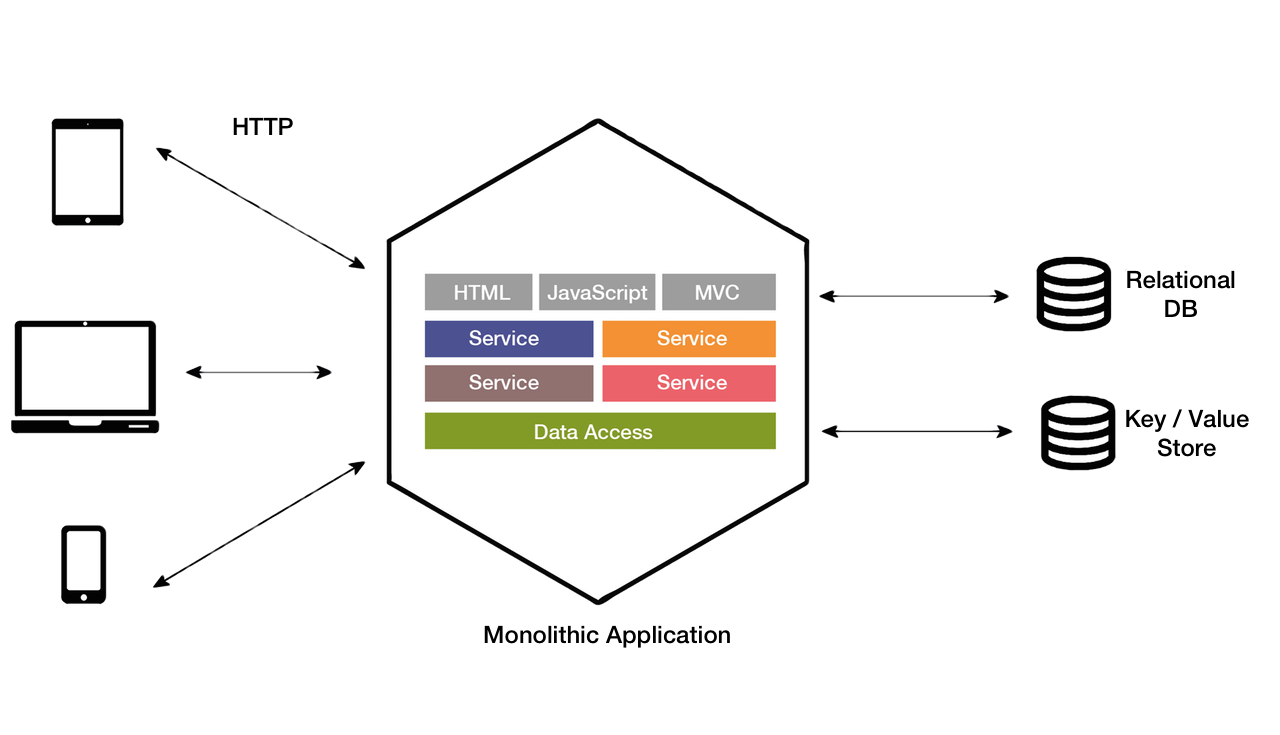
\includegraphics[scale=.2]{monolitFigure}
	\caption{Arhitectură Aplicație Monolit(imagine : http://bits.citrusbyte.com)}  
	\label{monolithicArhitecture}
  	\end{figure}
  	\section{Avantaje și dezavantaje}
  	\paragraph{}O aplicație monolit are mai multe avantaje in contextul unui business mic:
  	
  	\begin{itemize}
  	\item Faza de dezvoltare durează mai puțin timp, IDE-urile moderne reușind să genereze mult cod automat, ceea ce implică scădearea costurilor de producție.
  	\item Aplicația este usor de testat, automatizând procesul de testare a codului folosind o combinație de unit tests și integration test. 
  	\item Procesul de lansare în producție a unei aplicatii nu este complicat, deoarece este nevoie de rularea unei singure aplicații per server.
  	\end{itemize}
  	\paragraph{}Pe de altă parte, in momentul în care aplicația va creste ca și volum al codului, un număr mai mare de programatori vor trebui implicați în procesul de dezvoltare al aplicației, acest lucru nu este un lucru rău, doar ca aceștia vor intampina anumite impedimente:
  	\begin{itemize}
  	\item Cuplajul dintre componentele aplicației creste, iar acest fapt va îngreuna procesul de dezvoltare a unor noi functionalități, acest lucru va afecta timpul si costul necesar dezvoltării noii funcționalități.  
	\item Alegerea tehnologiilor folosite pentru dezvoltarea aplicației este permanentă.
	\item Integrarea/Intrarea unui programator in proiect va fi mai dificilă. Volumul aplicației fiind mare, va fi necesar un timp mai mare pentru înțelegerea tuturor funcționalităților si a decizilor luate pe proiect in trecut.
  	\end{itemize}
  	\paragraph{}Acestea sunt doar câteva dintre avantajele si dezavantajele unei aplicații monolit, dar sunt suficiente incât putem sublinia o idee generală. Aplicațiile bazate pe o arhitectura monolit sunt mai ușor de implementat în primă fază cu un cost mai redus, dar în momentul în care aplicația ajunge la un nivel mai avansat, este nevoie de o reconstruire parțiala sau totală a aplicației sau cel puțin este nevoie de o refactorizare care sa diminueze dezavantajele create de stilul arhitectural folosit. Majoritatea aplicațiilor încep ca și aplicații tip monolit, iar mai târziu se pot transaforma in aplicații cu arhitecturi bazate pe microservicii de exemplu.(\cite{thones2015microservices})
  \chapter{Arhitectura bazată pe servicii}
  	\section{Fundamentele arhitecturii bazate pe servicii}
  	\paragraph{}Unul din factorii care au dus la modificarea conceptelor despre cum trebuie să fie structurată o aplicație, a fost evolutia tehnologică rapidă și numărul tot mai ridicat de persoane care aveau acces la internet.
	\paragraph{}Arhitectura bazată pe servicii (în engleză „Servici Oriented Architecture”, prescurtat „SOA”), este un tip de arhitectură care s-a născut datorită nevoii tot mai mari de dezvoltare rapidă a cât mai multor funcționalități într-un timp cât mai scurt, si in paralel pe cât posibil.
	\paragraph{}Unul din motivele principale pentru apariția acestui stil arhitectural s-a datorat dorinție producătorilor ca o aplicație să poată sa fie folosită de pe diferite platforme. Dacă pentru fiecare platforma diferită era nevoie ca toată aplicația să fie rescrisă, costul ar fi fost prea mare, această soluție nu era plauzibilă. Datorită acestui fapt s-a decis că logica aplicației ar trebui să fie decuplată de partea din față a aplicației. În felul acesta, fiind necesară doar rescrierea  unei parți mult mai mici din aplicație pentru ca aceasta să poată functiona pe diferite tipuri de platforme. Odată cu această decizie, un nou stil arhitectural a apărut.
	\paragraph{}Pentru început, s-a incercat enunțarea a 8 principii, care ar trebui respectate intr-o arhitectură bazată pe servicii.
	\paragraph{}Acestea sunt:
	\begin{itemize}
	\item Serviciile sunt autonome.
	\item Serviciile sunt slab cuplate
	\item Serviciile trebuie să abstractizeaze logica pe care o folosesc.
	\item Serviciile împart un contract formal.
	\item Serviciile sunt compozabile
	\item Serviciile sunt refolosibile
	\item Serviciile nu au stare
	\item Serviciile se pot descoperii
	\end{itemize}
	\paragraph{}Din aceste 8 principii, primele 4 sunt cele mai importate, acestea reprezentând fundația arhitecturii bazate pe servicii. Toate cele 8 principii se suțin intre ele, dar primele 4 principii induc și restul.
  	\section{Principiile arhitecturii bazate pe servicii}
  	\subsection{Autonomia}
  	\paragraph{}Orietarea către servicii cere o atitudine serioasă atunci cand vine vorba de împărtirea lor in blocuri logice de sine stătătoare. Pentru ca serviciile sa fie fiabile și previzibile, trebuie sa se exercite un grad mai ridicat de control asupra resurselor pe care ele le folosesc.
  	\paragraph{}Odată cu cresterea nivelului de control al unui serviciu asupra propriului context de executie, se reduc dependințele din serviciu, ceea ce ne duce spre un alt principiu, cel al cuplajului slab. Chiar dacă exclusivitatea asupra logicii pe care un serviciu o encapsulează nu poate să fie deplină, principalul obiectiv este atribuirea unui nivel rezonabil de control asupra oricărei logici pe care o prezintă intr-un moment al executiei.
  	\paragraph{}Având in vedere că pot exista deferite metode de a masura autonomia, este bine facem distincție intre ele. Spre exemplu, un serviciu poate avea mai multe nivele de autonomie:
    \begin{itemize}
    \item Autonomie la nivelul serviciului
    \item Autonomie pură
    \end{itemize}
  	\subsection{Cuplajul slab}
  	\subsection{Abstractizarea}
  	\subsection{Contractul Formal}
  	\subsection{Șabloane de proiectare într-o arhitectură bazată pe servicii}
\chapter{Sabloane de proiectare bazate pe microservicii}
	\section{Sabloane de implementare a microservicilor}
		\subsection{Agregator}
		\subsection{API Gateway}
	\section{Sabloane arhitecturale de proiectare}
		\subsection{Service bus}
		\subsection{Procesare asincrona}
		\subsection{Agregarea proceselor}
		\subsection{Alte Sabloane}
\chapter{Studiu de Caz}
	\section{Introducere}
	\paragraph{}Netflix este o companie care a început prin a vinde sau închiria filme pe DVD-uri. Ulterior furnizând acces online la filme si seriale. Netflix fiind un gigant in industria televiziunii online. Aplicația netflix este o aplicație la scară mondială, care în momentul in care firma a horărat schimbarea arhitecturii avea un trafic de 8 milioane de utilizatori, ajungând la finalul anul 2018 la 139 de milioane de utilizatori.	
	\paragraph{}Dupa cum am discutat până acum, o arhitectură bazată pe microservicii nu are chiar o definiție propriu zisă, dar dupa cum susține Martin Fowler, microserviciile sunt implementarea corectă a arhitecturii bazate pe servicii.
	\paragraph{}În acest capitol vom cuprinde trecerea de la o arhitectură monolit la o arhitectura bazată pe servicii, motivele pentru care s-a facut aceasta tranziție, pașii prin care s-a facut aceasta trecere, avantajele cât si dezavantajele acestei treceri, cât si despre rezultatul final.
	\section{Tranziția către microservicii în compania Netflix}
	\paragraph{}În acest studiu de caz o să ne bazăm pe informațiile oferite de doua dintre personajele importante care au luat parte la tranziția catre microservicii:
	\begin{itemize}
	\item Ruslan Meshemberg
	\item Adrian Cockcroft	
	\item Josh Evans	
	\end{itemize}
	\subsection{Arhitectura aplicației de azi}
	\paragraph{}În următoarea diagrama, este reprezentată, arhitectura bazată pe microservicii a aplicației Netflix.
	\begin{figure}[h]
  	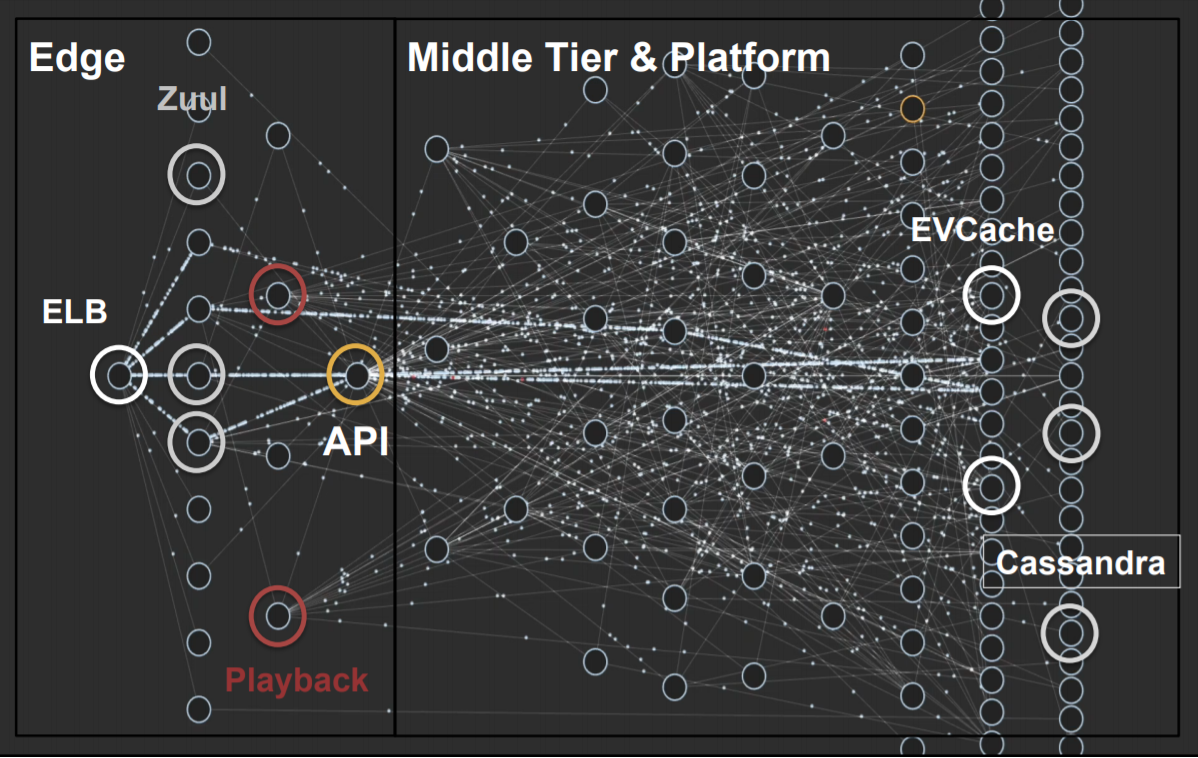
\includegraphics[scale=.651]{netflixarhitecuture}
	\caption{Arhitectura Aplicației Netflix()}  
  	\end{figure}
  	\paragraph{}Făcând o scurtă analiză asupra diagramei, putem să observam că prezentarea este una stratificată, nodul notat „ELB” rebrezintă un balansier de capacitate elastic (Elastic Load Balancer), care se o ocupă cu distrubuirea uniforma a cererilor catre microservicii. Stratul in care avem nodul notat „Zuul”, este un strat de tip proxy care ajută la oprirea atacurilor cibernetice. Iar zona dintre acest strat si „Middle Tier” este reprezentată de componente accesibile clientilor. În partea a 2-a a diagramei, este un strat destul de stratificat de microservicii care conțin mai multa logică si serversc componentelor din prima parte a diagramei. Ultimul strat, cel care contine si nodul notat cu „Cassandra” pe diagramă, reprezintă stratul de acces la bazele de date, datele fiind salvate separat in baza de date NoSQL. Iar intre ultimele 2 straturi   explicate, avem un strat care se ocupa de caching.
  	\paragraph{}O diagramă mai reprezentativă pentru arhitectura bazată pe microservicii a Netflix, care contine mai mult de 500 de microservicii este numita si diagrama de arhitectura „Death Star”(\ref{deathStarArhitecture}).
  	\paragraph{}Așadar, având în vedere scala la care știm deja ca funcționează aplicația Netflix, putem deja considera că arhitectura bazată pe microservicii isi servește bine scopul. În continuare vom discuta efectiv despre motivele, pașii, beneficiile și costurile acestei schimbari de arhitectură.
  	\begin{figure}[h]
  	\centering
  	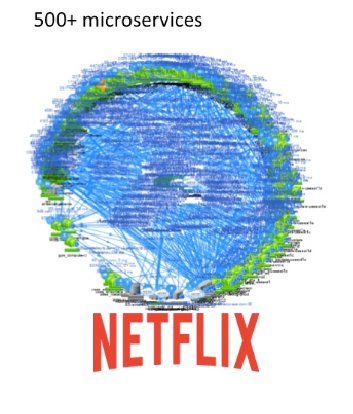
\includegraphics[scale=.8]{deathstararhitecture}
	\caption{Arhitectura Aplicației Netflix()}  
	\label{deathStarArhitecture}
  	\end{figure}
	\subsection{Motive}
	\paragraph{}Unul dintre primele motive care au înpins compania netflix să iși mute aplicația catre cloud și odata cu asta, inceperea tranziției către noua arhitectură, a fost o criză întampinată în 2008 când baza lor de date a fost coruptă, iar acest lucru a dus la intreruperea activitații timp de 3 zile. 
	\paragraph{}Al doilea motiv a fost ritmul alert în care compania crestea si numarul tot mai mare de utilizatori. Toată lumea era conștientă că numărul de utilizatori va creste si mai mult iar aplicația trebuia scalată din ce in ce mai mult.
	\paragraph{}În momentul în care vorbim de scalabilitate, putem sa ne gândim la asta in 2 feluri, scalare pe veriticala (termenul în engleză „scale up”) sau scalare pe orizontală (termenul în engleză „scale out”). Scalarea pe verticală poate fi văzută ca imbunătățirea constantă a sistemului, nevoia suplimentară de memorie, spatiu pe disk, puterea de procesare mai mare. Acest lucru este posibil doar pană la un anumit punct, ajungându-se la atingearea limitei tehnologice. În plus scalarea pe verticală devenind din ce in ce mai costisitoare.
	\paragraph{}Scalarea pe verticală a devenit în mod rapid, o soluție mult mai ușoară, acest tip de scalare presupune distribuirea aplicației pe mai multe sisteme care lucreaza împreuna. Așadar, în momentul în care aplicația trebuie scalată, este nevoie doar de introducerea unei noi componente in sistem si crearea unei noi instanțe pentru serviciul pentru care se doreste scalarea, iar având in vedere ca Netflix migra in același timp înspre cloud, activarea unei noi unitați si instanțierea unui nou serviciu se poate face foarte simplu și rapid.
	\paragraph{}Mergând mai departe, se dorește eliminarea tuturor punctelor critice, ceea ce înseamnă ca se dorește ca în sistem sa nu existe posibilitatea ca o eroare sa se propage, generând in cascadă și alte erori ale sistemului. Soluția agreeată pentru această problemă a fost crearea de servicii fara stare (în engleză „stateless”), aceestea având proprietatea că anumite date de intrare vor fi procesate si transformate în date de ieșire in același mod indiferent de instanța serviciului. Iar ca si testare a acestei idei, cei de la Netflix folosesc un tool numit „Chaos Monkey”, care aleator distruge cate o instanța al unui serviciu pentru a se garanta că o asemenea eroare nu este propagată în întreg sistemul. Ca acest concept să funcționeze, este nevoie de un balansier, pentru ca datele să fie redistribuite către o altă instanță a aceluiași serviciu.
	\begin{figure}[h]
  	\centering
  	
\includegraphics[scale=.5]{chaos}
	\caption{Chaos Monkey}  
	\label{chaosMonkey}
  	\end{figure}
	\subsection{Avantaje și dezavantaje, costuri și sacrificii}
	\paragraph{}Din punct de vedere al avantajelor pe care microserviciile le aduc, unul dintre ele a fost probabil cel mai apreciat de Netflix, a fost viteza de dezovolare a produsului. Acest lucru, probabil fiind datorat faptului că fiind primul care aduce o imbunătățire sau un lucru nou, este favorizat față de cei care il urmează. Așadar, microserviciile au permis o redistribuire a echipelor, iar noile echipe având responsabilitați separate, conceptul de a astepta dupa o altă echipă pentru a putea sa iti faci treaba, incepe sa dispară.
	\begin{figure}[h]
  	\centering
  	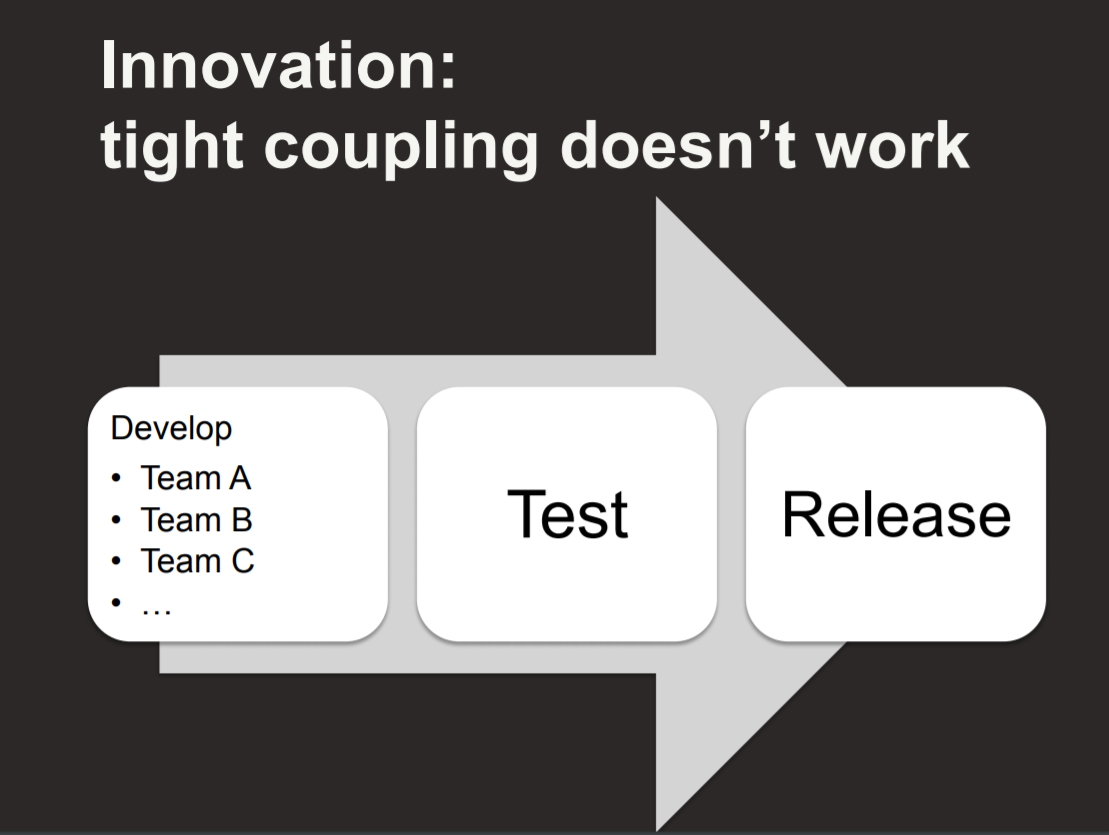
\includegraphics[scale=.25]{tightCoupling}
	\caption{Procesul de dezovoltare intr-o aplicație monolit}  
	\label{tightCoupling}
  	\end{figure}
  	\begin{figure}[h]
  	\centering
  	\includegraphics[scale=.25]{looseCoupling}
	\caption{Procesul de dezovoltare intr-o aplicație bazată pe microservicii}  
	\label{looseCoupling}
  	\end{figure}
  	\paragraph{}După cum se poate observa în prima figură (\ref{tightCoupling}), în prima parte trebuie ca toata aplicația să fie dezvoltată, apoi testată si apoi lansată. Iar în a doua figura (\ref{looseCoupling}), se poate observa ca echipele pot să lucreze fiecare în ritmul lor, nefiind nevoiți să depindă constant de restul. Microserviciile nefiind nevoite să fie lansate in execuție împreună.
	\paragraph{}Pe de altă parte, trebuie să avem in vedere faptul că în această schimbare au fost nevoie și de sacrificii, unele referindu-se la costuri, altele la relație oamenilor din echipe. Printre aceastea se pot numară urmatoarele:
  	\begin{itemize}
  	\item În primul rând, costul de dezvoltare si mentenanță a aplicație a crescut. Motivul fiind următorul: tranziția a fost una de durată, iar in timp ce se crea aplicația cu noua arhitectură, aplicația monolit trebuia sa ramână in picioare. Și pe de alta parte, datele trebuiau sa fie replicate si salvate atat in aplicația noua cât si in cea curentă.
  	\item În al doilea rând, tehnologiile din noua aplicație s-au schimbat partial fața de aplicația monolit, iar compania trebuie sa suporte toate tehnologiile existente din ambele proiecte. Un exemplu este legat de bazele de date, in aplicația monolit existând baze de date relaționale, iar bazele de date din microservicii au devenit baze de date NoSQL. Mai târziu un evoluția noi arhitecturi vor aparea microservicii scrise si in NodeJS, Phyton si alte limbaje de programare.
    \item În al treilea rand, un alt compromis, poate nu atat de mare, a fost în momentul în care compania a ales să traiască intr-o zonă hibridă, asta insemnând ca au inceput sa exite servicii scrise in diferite limbaje de programare cum are fi NodeJS, Phyton si altele. Acest lucru fiind posibil atât timp cât era respectat un format pentru datele de intrare cât și pentru datele ieșire.
  	\item În ultimul rând, un alt compromis care a trebuit făcut a fost schimbarea structurii echipelor. De la echipe specializate pe dezvoltare, echipe specializate pe testare si echipe specializate in lansarea aplicației in mediul online, s-a ajuns la echipe mai mici care să se ocupe de intreg ciclul de viată al unui microserviciu(\ref{endtoend}), De la implementare, pâna la lansarea lui in execuție.
  	\end{itemize}
  	\begin{figure}[h]
  	\centering
  	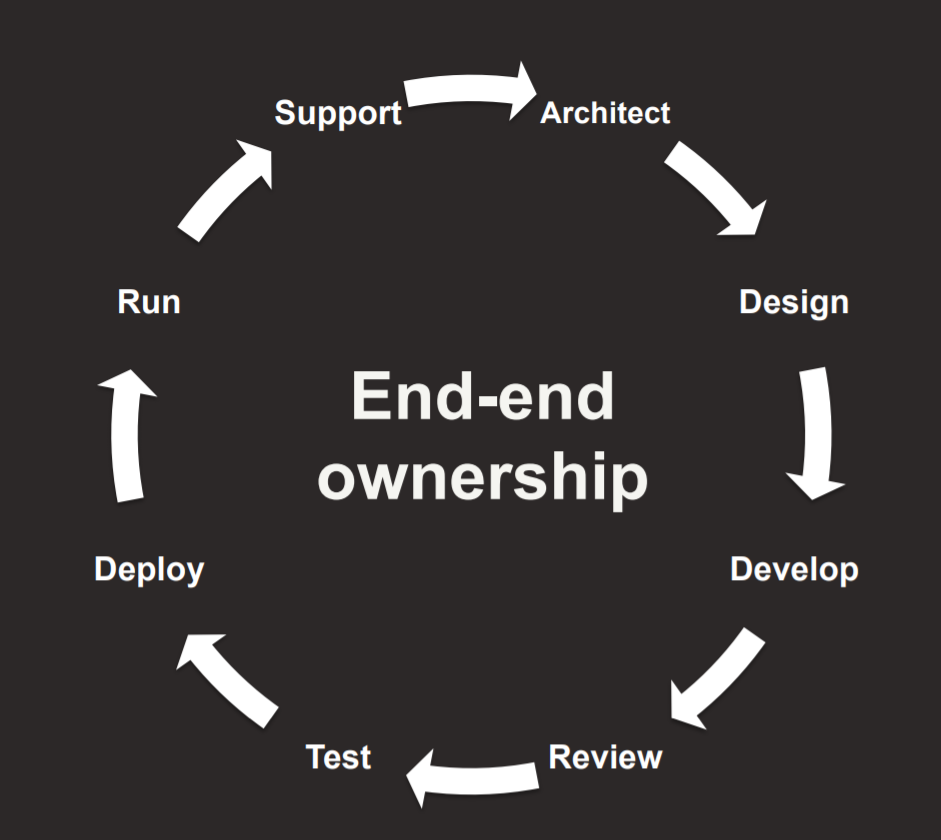
\includegraphics[scale=.7]{endtoend}
	\caption{Ciclul de viață al unui microserviciu}  
	\label{endtoend}
  	\end{figure}
  	\subsection{Descrierea tranziției catre microservicii}
  	\paragraph{}Unul din cei mai importanți oameni care a ajutat la tranziția aplicație catre microservicii si mutarea acesteia in cloud, este specialistul în scalabilitate de la Netflix, Adrian Cockcroft. Dupa cum am amintit și mai sus, posibilitățile de scalare erau pe verticală si pe orizontală. Dupa cum Adrian Cockcroft a susținut in timpul unei conferințe, scalarea pe verticală ar fi însemnat în momentul acela, anul 2009, construirea unui nou centru de date (în engleză „data center”) cu un cost estimativ de aproximativ 100 de milioane de dolari. Iar pe aceași tema, a glumit, spunând ca banii respectivi ar fi mai bine folosiți daca Netflix ar cumpăra inca un sezon din „House Of Cards”(acesta fiind un serial TV). Soluția plauzibilă care a rămas, fiind scalarea pe orizontală.
  	\paragraph{}Primul pas fiind de test, s-a încercat mutarea unui serviciu in cloud, iar alegerea nu a fost intâmplătoare, a fost ales un serviciu care să nu fie in prima linie pentru utilizator, adică un serviciu care mai mult procesează cantităti mari de date in spate. Spre exemplu, algoritmul folosit pentru auto completarea câmpului de cautare. După ce acest pas a fost realizat cu succes, si serviciul era folosit de aplicația monolit, procesul a continuat.
  	\paragraph{}Un alt pas important a fost schimbarea bazei de date, de la baze de date relaționale Oracle, la baza de date NoSQL („Cassandra”). Acesta bază de date este folosită și acum pentru aplicația Netflix. Având în vedere ca este open source(în engleza „open sourse”), Netflix a dezvoltat un feature care ajuta la replicarea usoară a datelor.
  	\paragraph{}După ce întreaga tranziție a fost gata, dupa anul 2012, multe dintre soluțiile aplicate in timpul tranziției au fost publicate, sursele devenind surse deschise.
	\paragraph{}Așadar succesul Netflix se datorează in mare parte lui Adrian Cockcroft, care este un vizionar, reusind tranziția Netflix catre o arhitectura bazată pe microservicii in cloud, intr-un moment in care nimeni nu dorea să creadă ca cloud-ul ar putea să fie o soluție(\ref{toCloud}).
	\begin{figure}[h]
  	\centering
  	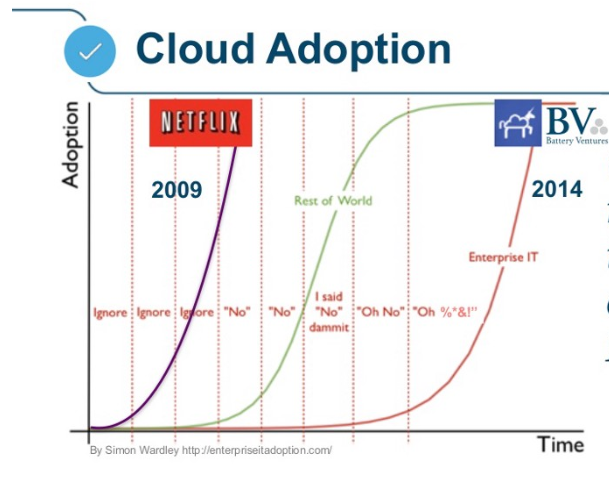
\includegraphics[scale=.7]{toCloud}
	\caption{Migrarea catre cloud a aplicațiilor}  
	\label{toCloud}
  	\end{figure}
\chapter{Aplicație Practica}
	\section{Cerința}
	\section{Specificații}
	\section{Arhitectura aplicatiei}
	\section{Implementare}
	\section{Sablone bazate pe microservicii in practica}
\chapter{Concluzii}

\bibliographystyle{apacite}
\bibliography{referinte}

\begin{flushleft}
\textbf{Cockcroft, Adrian. 2015. \texttt{Talking microservices with the man who made Netflix’s cloud famous. [interviu cu] Derrick Harris. 2015.}}
\end{flushleft}

\begin{flushleft}
\textbf{
Cockroft, Adrian. 2014. \texttt{Migrating to Microservices by Adrian Cockroft. YouTube. [Interactiv] 2014. https://www.youtube.com/watch?v=1wiMLkXz26M.}}
\end{flushleft}

\begin{flushleft}
\textbf{
Erl, Thomas. 2009. \texttt{SOA Design Patterns. Crawfordville Indiana : Prentice Hall, 2009.}}
\end{flushleft}

\begin{flushleft}
\textbf{
Fowler, Martin. 2014. \texttt{Microservices, 2014,. MartinFowler.com. [Interactiv] 2014. https://martinfowler.com/articles/microservices.html.}}
\end{flushleft}

\begin{flushleft}
\textbf{
OASIS Foundation. 2006. \texttt{Reference Model for Service Oriented Architecture. [Interactiv] 2006. https://docs.oasis-open.org/soa-rm/v1.0/soa-rm.html.}}
\end{flushleft}



\end{document}
